
\title{RECENT DEVELOPMENTS IN HODGE THEORY: A DISCUSSION OF TECHNIQUES AND RESULTS}
\markright{RECENT DEVELOPMENTS IN HODGE THEORY: A DISCUSSION OF TECHNIQUES AND RESULTS}

\author{By~ PHILLIP GRIFFITHS and WILFRIED SCHMID}
\markboth{PHILLIP GRIFFITHS and WILFRIED SCHMID}{RECENT DEVELOPMENTS IN HODGE THEORY: A DISCUSSION OF TECHNIQUES AND RESULTS}

\date{}
\maketitle

%\setcounter{page}{21}
\setcounter{pageoriginal}{20}


\section*{Introduction}\label{art4-sec1}
In\pageoriginale this paper, we shall review several recent developments in \textit{Hodge theory}, as applied to the study of the cohomology of algebraic varieties. In some sense, we are continuing the report \cite{art4-key21} of the first author, in which the then current work in Hodge theory was discussed without proof and a number of open problems were raised. Here we shall be concerned primarily with \textit{methods of proof}, \iec understanding in as transparent terms as possible the techniques utilized in this recent work in Hodge theory. We shall also present some results, due to the second author \cite{art4-key41}, which have just now been published, and shall bring up to date the status of the problems raised in \cite{art4-key21}.

One of the recent developments we shall discuss is Deligne's theory of \textit{mixed Hodge structures} (\cite{art4-key12}, \cite{art4-key}, \cite{art4-key14}). In this work, Deligne extends classical Hodge theory first to open, smooth varieties \cite{art4-key13}, then to complete, singular varieties \cite{art4-key14}, and finally to general varieties, also in \cite{art4-key14}. The heuristic reasoning explaining why such a theory should be possible is given in \cite{art4-key12}.

Deligne's technique is to use \textit{resolution of singularities} \cite{art4-key29}, in order to be able in each case to write the cohomology of the variety in question as being derived from the cohomology of K\"ahler manifolds by homological algebra. Typically this process gives the cohomology of the variety as the abutment of a spectral sequence whose $E_1$ or $E_2$ term is the cohomology of a smooth projective variety. Thus the $E_1$ or $E_2$ term has a \textit{Hodge structure}, and in order for this structure to survive as a Hodge structure on $E_\infty$, inducing the desired mixed Hodge structure on the cohomology of the variety, it is necessary that the spectral sequence degenerates. Following a discussion of the formalism of Hodge structures and mixed Hodge structures in \S 1, we have in \S 2 (a), \S 4, and \S 5 (d)  presented several typical degeneration arguments in as direct a manner as we could.

In \S \ref{art4-sec4} we construct the mixed Hodge structure on the cohomology of the simplest singular complete varieties, namely those having only \textit{normal crossings as singularities}. Here the main reason for the various degeneration theorems can be clearly isolated. The result in \S \ref{art4-sec4} stops far short of proving the existence of a mixed Hodge structure on the cohomology of a general singular variety \cite{art4-key14}. However, it is the method by which one most frequently \textit{calculates} this mixed Hodge structure (cf. \cite{art4-key10}, for instance), once it is known to exits.

In \S \ref{art4-sec5}, we have reproved the main result in the open case \cite{art4-key13} from a more analytic and less homological point of view. Our main idea is, instead of using the customary de Rham complex of $C^\infty$ forms on a compact K\"ahler manifold, to utilize a larger complex containing $L^1$-forms with certain precise types of singularities, and where the \textit{Gysin map} can be given on the form level preserving the Hodge filtration. This complex is discussed in \S\ref{art4-sec2}(b), where it is pointed out that the introduction of singular forms is necessary in order to have such a Gysin map on the form level. Operating inside this complex allows us to see clearly the differentials in the relevant spectral sequence in the open case, and to conclude the degeneracy result from the principle of two types (\S\S\ref{art4-sec5}(d), (e)).

Section 6 is devoted to some applications of Deligne's theory. First in \S \ref{art4-sec6}(a), we give his ``theorem on the fixed part'', which is the main tool in Deligne's study of the moduli of Hodge structures. Then, in \S\ref{art4-sec6}(b), we give a direct proof of an interesting result from \ref{art4-13}, concerning meromorphic differential forms on algebraic verieties; and finally we discuss an application of mixed Hodge structures to \textit{intermediate Jacobians} in \S \ref{art4-sec6}(c).

The second technique which we shall explore in some depth is the use of \textit{hyperbolic complex analysis}, as it applies to variation of Hodge structure. Hyperbolic complex analysis is the study of the influence of \textit{negative curvature} on holomorphic mappings. The classifying spaces for variation of Hodge structure are negatively curved, relative to the holomorphic maps which might arise in algebraic geometry (\cf. \cite{art4-key11}, \cite{art4-key25}, and \S \ref{art4-sec3}(a), (b)), and so it is natural to apply the general philosophy in this case.

Following a discussion of the basic \textit{Ahlfors lemma} and its variants in \S \ref{art4-sec7}(a), we have given Borel's proof of the quasi-unipotence of the \textit{Picard-Lefschetz transformation} in \ref{art4-sec7}(b); this should illustrate in a simple fashion the power of the method.

Perhaps the most penetrating use of the philosophy of hyperbolic complex analysis occurs in the \textit{Nevanlinna theory} \cite{art4-key24}, which affords a general mechanism for analyzing the singularities of a holomorphic mapping. Following a preliminary result from Nevanlinna theory in \S \ref{art4-sec8}(a), we have used this technique to give rather simple, geometric proofs of \textit{Borel's extension theorem} \cite{art4-sec5} in \S \ref{art4-sec8}(b), and of the \textit{Riemann extension theorem for variation of Hodge structure} \cite{art4-key19} in \S \ref{art4-sec8}(c).

A final recent development we shall discuss is the work by the second author \cite{art4-key41} and joint work by him and Clemens \cite{art4-key10}, concerning the asymptotic behavior of the Hodge structures on the cohomology groups of an algebraic variety as it acquires singularities. In \S \ref{art4-sec9}(a), we have used the theorem on \textit{regular singular points} (\S \ref{art4-sec3} (c)), together with the Ahlfors lemma, to give an alternate proof of the first theorem from \cite{art4-sec41}. This result, the \textit{nilpotent} orbit theorem, reduces the case of a general degeneration of Hodge structure to the study of a special king a \textit{nilpotent orbit} in a classifying space for variation of Hodge structure. It seems possible to use Nevanlinna theory in place of the theorem on regular singular points to prove the same result, but we have not purshed this here.

The second main theorem from \cite{art4-key41}, the $SL_2$-\textit{orbit theorem}, gives a detailed and somewhat technical description of the nilpotent orbits which can come up when a one-parameter family of Hodge structures degenerates. The proof depends heavily on Lie theory. In \S \ref{art4-sec9}(b), besides stating the theorem, we describe the observations which originally led to the proof, as well as to the statement, of the theorem.

Some applications of these two theorems will be mentioned in \S\ref{art4-sec10}; we also summarize joint results of Clements and the second author about the topology of a degenerating family of projective manifolds, which again are partly based on the two theorems.

We conclude with an appendix, reviewing the current status of the problems and conjectures contained in the report \cite{art4-sec21} of the first author.

\section{Basic definitions}\label{art4-sec1}
(a)~ \textit{Hodge structures.} Let $H_{\bR}$ be a finite dimensional real vector space, containing a lattice $H_{\bZ}$, and let $H=H_{\bR} \otimes_{\bR} \bC$ be its complexification.

\begin{definition}\label{art4-def1.1}
`A Hodge structure of weight $m$' on $H$ consists of a direct sum decomposition
$$
H = \bigotimes_{p+q=m} H^{p,q}, \text{ with } H^{q,p} = \bar{H}^{p,q}
$$
\end{definition}

(Barring denotes complex conjugation.)

\begin{remark*}
The prototypical example is the decomposition according to Hodge type of the $m$-th complex cohomology group of a compact K\"ahler manifold. In this case, $m$, $p$, $q \;\geqslant 0$; however, it will be convenient to admit also negative values for $m$, $p$, and $q$. For example, the \textit{Hodge structure of Tate} $T$(1) is defined by
$$
H_{\bZ} =\bZ, \; H_{\bR} = \bR, \; H = \bC, \; m= -2, \text{ and } H = H^{-1,-1}.
$$

For any two Hodge structures $H, H'$, both of weight $m$, the direct sum $H\oplus H'$ carries an obvious Hodge structure, also of weight $m$. Similarly, if $H$ and $H'$ have possibly different weight $m$ and $m'$,
$$
H\otimes H', \; \Hom (H, H'), \Lambda^p H, \; H^\ast
$$
inherit Hodge structures of weight $m+ m'$, $m'-m$, $pm$, and $-m$, respectively: $\lambda \in \Hom(H, H')$ has Hodge type $(p,q)$ if $\lambda(H^{r,s}) \subset (H')^{p+r, \; q+s}$ for all $r, s$; in particular, this definition applies to $H^\ast = \Hom (H, \bC)$, with $\bC$ carrying the trivial Hodge structure of weight $0; H \otimes H'$ can be identified with $\Hom (H^\ast, H')$, and $\otimes^pH$ induces a Hodge structure on its subspace $\Lambda^p H$.
 \end{remark*}

\begin{definition}\label{art4-def1.2}
A linear map $\varphi: H \to H'$ between vector spaces with Hodge structures will be called a morphism (of Hodge structures) if it is defined over $\bQ$, relative to the lattices $H_{\bZ}$, $H'_{\bZ}$, and if $\varphi (H^{p,q}) \subset (H')^{p,q}$, for all $p,q$. More generally, $\varphi$ is a morphism of type $(r,r)$ if again it is defined over $\bQ$, and if it has type ($r, r$) when viewed as an element of $\Hom(H, H')$.
\end{definition}

As a trivial, but nevertheless important, observation we note that morphism of type $(r,r)$ must vanish unless the weights $m$ and $m'$ of $H$ and $H'$ satisfy $m'=m+2r$.

To\pageoriginale each Hodge structure $H = \oplus_{p+q =m} H^{p,q}$ of weight $m$ one associates the \textit{Hodge filtration}
\setcounter{equation}{2}
\begin{equation}
H \supset \ldots \subset F^{p-1} \supset F^p \subset F^{p+1} \supset \ldots \supset 0 \text{ with } F^p = \oplus_{i \geqslant p} H^{i, m-i}.  \label{art4-eq1.3}
\end{equation}

It may be convenient to visualize the definition by means of the picture below:
\begin{figure}[H]
\centering
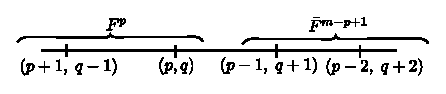
\includegraphics{art4-fig1.eps}
\end{figure}

The Hodge filtration determines the Hodge structure completely, since
\begin{equation}
H^{p,q} = F^p \cap \bar{F}^q \label{art4-eq1.4}
\end{equation}

Conversely, a descending filtration $\{F^p\}$ of $H$ arises as the Hodge filtration of some Hodge structure of weight $m$ if and only if
\begin{equation}
F^p \oplus \bar{F}^{m-p+1} \xrightarrow{\approx} H, \;\; \text{ for all } p.
\label{art4-eq1.5}
\end{equation}

Thus one has a 1:1 correspondence between Hodge structures and Hodge filtrations, \iec filtrations satisfying \eqref{art4-eq1.5}.

In terms of this latter description, a linear map $\varphi: H \to H'$, which shall be defined over $\bQ$, becomes a morphism of type $(r, r)$ exactly when it preserves the Hodge filtration, with a shift by $r$; in other words, when 
\begin{equation}
\varphi (F^p) \subset F'^{p+r}, \;\text{ for all }p. \label{art4-eq1.6}
\end{equation}

Now let $\varphi$ be a morphism of type $(r, r)$, $v$ a vector in $F'^{p+r} \cap \Iim \varphi$. By decomposing a vector in the inverse image of $v$ according to Hodge type, one finds that $v$ lies in the image of $F^p$. Thus:

a morphism of Hodge structures of type $(r,r)$ preserves the Hodge filtrations strictly, with a shift by $r$, in the sense that 
\begin{equation}
\varphi(F^p) = F'^{p+r} \cap \Iim \varphi, \text{ for all } p. 
\label{art4-eq1.7}
\end{equation}

We consider a Hodge structure $H = \oplus_{p+q = m} H^{p,q}$ and a bilinear form $Q$ on $H$, which shall be defined over $\bQ$. Also $Q$ shall be symmetric if $m$ is even, skew if $m$ is odd.

\setcounter{definition}{7}
\begin{definition}\label{art4-def1.8}
The Hodge structure is polarized by $Q$ if 
$$
\begin{matrix}
Q (H^{p,q} , H^{p', q'} =0) & \text{ unless } p = q', \; q = p',\\[2pt]
(\sqrt{-1})^{p-q} Q (v, \bar{v}) > 0 & \text{ for } v \in H^{p,q}, \; v \neq 0.
\end{matrix}
$$
\end{definition}

Apparently, the polarization form $Q$ must be nondegenerate. The Weil operator $C: H \to H$ of the Hodge structure is defined by 
\setcounter{equation}{8}
\begin{equation}
C_v = (\sqrt{-1})^{p-q} v, \text{ for } v \in H^{p,q} . \label{art4-eq1.9}
\end{equation}
In terms of the Hodge filtration and the Weil operator, the two conditions in \ref{art4-def1.8} become equivalent to 
\begin{equation}
\left.
\begin{matrix}
Q (F^p, F^{m-p+1}) = 0\\
Q (C v, \bar{v}) >0 \;\text{  for } v \neq 0.
\end{matrix}\right\}
\label{art4-eq1.10}
\end{equation}

The example we have in mind is the Hodge bilinear form on the primitive part of the cohomology of a smooth, projective variety over $\bC$, as will be discussed below.

It should be mentioned that the operations of tensor product, Hom exterior product, and duality can also be performed in the context of polarized Hodge structures. For example, if $Q$ and $Q'$ are polarization forms for Hodge structures $H$ and $H'$, then the induced bilinear form on $H \otimes H'$ polarizes the product Hodge structure.

\medskip
\noindent
(b)~ \textit{Mixed Hodge structures.} The symbols $H$, $H_{\bR}$, $H_{\bZ}$ shall have the same meaning as in the previous section.

\begin{definition}\label{art4-def1.11}
`A mixed Hodge structure' on $H$ consists of two filtrations,
$$
0 \subset \ldots \subset W_{m-1} \subset W_m \subset W_{m+1} \subset \ldots \subset H,
$$
the `weight filtration' which shall be defined over $\bQ$, and 
$$
H \supset \ldots \supset F^{p-1} \supset F^p \supset F^{p+1} \supset \ldots \supset 0,
$$
the `Hodge filtration', such that the filtration induced by the latter on $Gr_m(W_\ast) = W_m/W_{m-1}$ defines a Hodge structure of weight $m$, for each $m$ (the induced filtration on $Gr_m(W_\ast)$ is given by
$$
F^p (Gr_m (W_\ast)) = W_m \cap F^p/W_{m-1} \cap F^p).
$$
\end{definition}


\begin{remark*}
The notion\pageoriginale of a mixed Hodge structure contains that of a Hodge structure of weight $m$ as a special case; as Hodge filtration one takes the Hodge filtration in the old sense, and the weight filtration is defined by $W_m = H$, $W_{m-1} = 0$.
\end{remark*}

According to the definition of a mixed Hodge structure, only the successive quotients of the weight filtration have direct sum decompositions according to Hodge type. However, the following lemma of Deligne \cite{art4-key13} provides a more subtle global decomposition of $H$. For any pair of integers $(p,q)$, we consider the subspace
\begin{multline*}
I^{p,q} = (F^p \cap W_{p+q}) \cap (\bar{F}^q \cap W_{p+q} + \bar{F}^{q-1} \cap W_{p+q-2} +\\
 + \bar{F}^{q-2} \cap W_{p+q-3} + \ldots).
\end{multline*}
It is certainly not the case that $I^{p,q} = I^{q,p}$, but one does have the congruence $I^{p,q} \equiv I^{q,p} \mod W_{p+q-2}$, as will follow from the proof of lemma \ref{art4-lem1.12} below. This congruence $I^{p,q} \equiv \bar{I^{q,p}} \mod  W_{p+q-2}$ explains why every mixed Hodge structure with a weight filtration of length two splits over $\bR$, into a sum of two Hodge structures of pure weight. This splitting, of course, may be incompatible with the rational structure. As soon as the weight filtration has length greater than two, a ``general'' mixed Hodge structure will not split over $\bR$.

\setcounter{lemma}{11}
\begin{lemma}[\cf. Lemma 1.2.8 of \cite{art4-key13}.]\label{art4-lem1.12}
Under the projection $W_m \to Gr_m (W_\ast), \; I^{p,q}$, with $p+q=m$, maps isomorphically onto the Hodge subspace $Gr_m (W_\ast)^{p,q}$. Moreover,
$$
W_m = \oplus_{p+q\leqslant m} I^{p,q},
$$
and 
$$
F^p = \oplus_{i \geqslant p} \oplus_q I^{p,q}.
$$
\end{lemma}

\begin{proof}
In view of \eqref{art4-eq1.5}, the definition of a mixed Hodge structure amounts to the following:
\begin{align*}
& \text{given any $v \in W_n$ and integers $p,q$, with $p+q=m+1$,}\\
& \text{one can write $v = v'+\bar{v}'' + u $, such that $v' \in F^p \cap W_m$,}\\
& \text{$v'' \in F^q \cap W_m$, and $u\in W_{m-1}$; this decomposition is unique}\\
& \text{modulo $W_{m-1}$}. \tag{$\ast$}\label{art4-eq*}
\end{align*}

In order to prove the first assertion of the lemma, we fix $m$, $p$, $q$, subject to $m=p+q$, and $\alpha \in Gr_m (W_\ast)^{p,q}$. Then $\alpha$ can be represented by some\pageoriginale $v_0\in F^p \cap W_m$, and also by some $\bar{u}_0 \in \bar{F}^q \cap W_m$. Both are unique upto $W_{m-1}$, and $v_0 = \bar{u}_0 + w_0$, for some $w_0 \in W_{m-1}$. By induction on $k$, starting with $k=0$, we shall find vectors
\begin{gather*}
v_k \in F^p \cap W_m, \qquad w_k \in W_{m-1-k}\\
u_k \in F^q \cap W_m + F^{q-1} \cap W_{m-2} + F^{q-2} \cap W_{m-3} + \ldots + F^{q+1-k} \cap W_{m-k}
\end{gather*}
which will be unique up to $W_{m-k}$, such that $v_k$ represents $\alpha$, and $v_k = \bar{u}_k + w_k$. For $k=0$, this has been done $(F^{q+1} \subset F^q !)$.  If $v_k$, $u_k$, $w_k$ have been picked, we apply \eqref{art4-eq*} to $w_k$: we write $w_k = w'_k + \bar{w}''_k + w_{k+1}$, with $w'_k \in F^p \cap W_{m-1-k}$, $w_k \in F^{p-k} \cap W_{m-1-k}$, $w_{k+1} \in W_{m-2-k}$, uniquely modulo $W_{m-2-k}$. The vectors $w_{k+1}, \; v_{k+1} = v_k - w'_k$, $u_{k+1} =  u_k + w''_k$ then have the desired properties. For large enough $k$, $W_{m-1-k} = 0$; hence $\alpha$ has a unique representative in $I^{p,q}$. We may deduce that
$$
W_m = W_{m-1} \oplus (\oplus_{p+q=m} I^{p,q}),
$$
and thus $W_m = \oplus_{p+q\leqslant m} I^{p,q}$. As for the last statement of the lemma, the sum of the $I^{p,q}$ is now known to be direct. Also, one containment is obvious. We consider some $v \in F^p$, and we let $m$ be the least integer for which $v \in W_m$. The image of $v$ in $Gr_m (W_\ast)$ has Hodge components of type $(i, m-i)$, with $i \geqslant p$, because $v \in F^p \cap W_m$. Subtraction off components in the spaces $I^{i,m-i}$, with $i \geqslant p$, we can push $v$ into $W_{m-1}$. Continuing with descending induction on $m$, we find that $v \in \oplus_{i \geqslant p} \oplus \oplus_q I^{i,q}$, as was to be shown.
 
A \textit{morphism} between two mixed Hodge structures $\{H, W_m, F^p\}$,\break $\{H', W'_m, F'^p\}$ is a rationally defined linear $\map \varphi; H \to H'$, such that $\varphi(W_m) \subset W'_m$ and $\varphi (F^p) \subset F'^p$. More generally, a rationally defined linear $map \varphi : H \to H'$ will be called a morphism of mixed Hodge structures of type $(r,r)$ if $\varphi (W_m) \subset W'_{m+2r}$, $\varphi (F^p) \subset F'^{p+r}$, for all $p$ and $m$. In this case, the induced mapping
$$
\varphi: Gr_m (W_\ast) \to Gr_{m+2r} (W'_\ast)
$$
becomes a morphism of type $(r,r)$ relative to the two Hodge structures of weights $m$ and $m+ 2r$, respectively.
\end{proof}

\setcounter{lemma}{12}
\begin{lemma}\label{art4-lem1.13}
A morphism\pageoriginale of type $(r,r)$ between mixed Hodge structures is strict with respect to both the weight and Hodge filtrations, with the appropriate shift in indices. More precisely, $\varphi (W_m) = W'_{m+2r} \cap \Iim \varphi, \; \varphi (F^p) = F'^{p+r} \cap \Iim \varphi$.
\end{lemma}

\begin{proof}
The definition of the subspaces $I^{p,q}$ immediately gives the containments $\varphi(I^{p,q}) \subset I'^{p+r, q+r}$. Now let $v \in W'_{m+2r} \cap \Iim \varphi$, so that $v = \varphi (u)$ for some $u \in H$. According to \ref{art4-lem1.12},
$$
u = \sum_{p,q} u^{p,q}, \text{ with } u^{p,q} \in I^{p,q}.
$$
Then $\varphi (u^{p,q}) \in I'^{p+r , q+r}$, and $v =\sum_{p,q} \varphi (u^{p,q}) =in W'_{m+2r}$. Again appealing to \ref{art4-lem1.12}, we deduce that $\varphi(u^{p,q}) =0$, unless $p+q \leqslant m$. Hence
$$
v = \varphi \left(\sum_{p+q \leq m} u^{p,q} \right) \in \varphi (W_m).
$$

The case of the Hodge filtration is treated similarly.
\end{proof}

\begin{lemma}\label{art4-lem1.14}
Let $\varphi: H \to H'$ be a morphism of mixed Hodge structures of type $(r,r)$. Then the induced Hodge and weight filtrations put mixed Hodge structure both on the kernel and the cokernel.
\end{lemma}

\begin{proof}
As for the kernel, given $v \in \ker \varphi \cap W_m$ and any integer $p$, we must exhibit vectors
$$
v'\in \ker \varphi \cap W_m \cap F^p, \; v'' \in \ker \varphi \cap W_m \cap F^{m-p+1}, \; w \in \ker \varphi \cap W_{m-1},
$$
such that $v = v' + \bar{v}''+u$, and these must be uniquely determined modulo $\ker \varphi \cap W_{m-1}$. The uniqueness already follows from the corresponding statement about $H$. Also, there do exist $u'\in W_m \cap F^p$, $u'' \in W_m \cap F^{n-p+1}$, such that $v \equiv u' + \bar{u}'' \mod W_{m-1}$. Since $\varphi(v) = 0$, we conclude that $\varphi (u')$, $\varphi (u'') \in W'_{m+2r-1}$. By appealing to \ref{art4-lem1.12} and decomposing $u'$ into its components in the subspaces $I^{s,t} \subset H$, we can find $u'_1 \in W_{m-1} \cap F^p$, so that  $\varphi(u') = \varphi(u'_1)$. Similarly, $\varphi (u'') = \varphi (u''_1)$ for some $u''_1 \in W_{m-1} \cap F^{m-p+1}$. The vectors $v'= u'-u'_1$, $v''=u'' - u''_1$, $w = v - v'-\bar{v}''$ have the desired properties. In order to prove the assertion about the cokernel, one only has to check one nontrivial fact: if $u \in W'_m \cap F'^p$, $v \in W'_m \cap F'^{m-p+1}$, and if $u + \bar{v} \in w'_{m-1} +\Iim \varphi$, then $u, v\in W'_{m-1} + \Iim \varphi$. Using \ref{art4-lem1.12}, this can be done, in a manner similar to the argument above. Details are left to the reader.
\end{proof}

\setcounter{coro}{14}
\begin{coro}\label{art4-coro1.15}
Let $(H^\ast, d)$ be a finite dimensional complex with a mixed Hodge structure, and such that the differential $d$ is a morphism of mixed Hodge structures of type $(r,r)$, for some $r$. Then in induced filtrations on the cohomology determine a mixed Hodge structure.
\end{coro}

As a final remark, whose verification is left to the reader, we want to add the 

\setcounter{observation}{15}
\begin{observation}\label{art4-obser1.16}
Let $0 \to H' \to H \to H'' \to 0$ be an exact sequence of vector spaces. If two filtrations $\{W_l\}$ and $\{F^p\}$ for $H$ induce mixed Hodge structures on both $H'$ and $H''$, then they determine a mixed Hodge structure on $H$ itself.
\end{observation}

\section{Classical Hodge theory}\label{art4-sec2}
(a)~ \textit{The cohomology of a K\"ahler manifold}. Let $V$ be a compact, complex manifold of dimension $n$, and $A^\ast (V)$ the de Rham complex of $C^\infty$ forms on $v$. The decomposition into type
$$
A^\ast (V) = \oplus_{p,q} A^{p,q} (V)
$$
reflects the complex structure on $V$, and \textit{via} de Rham's theorem has implications in the cohomology $H^\ast (V, \bC)$. However, not very much is known about this unless $V$ is K\"ahler, or at least nearly K\"ahler. In this case, there are two main sources for the many profound implications which the complex structure plus the K\"ahler metric have in the coholomogy, and we shall briefly discuss these.

Suppose that $ds^2_V = \Sigma_{i,j} g_{ij} dz_i dz_j$ is a K\"ahler metric with fundamental (1,1)-form $\omega = \dfrac{\sqrt{-1}}{2} \Sigma_{i,j} g_{ij} dz_i \wedge d\bar{z}_j$. The operators 
\begin{align*}
& L: A^k (V) \to A^{k+2} (V)\\ 
& \wedge : A^k (V) \to A^{k-2} (V)
\end{align*} 
are defined by $L (\varphi) = \omega \wedge \varphi$ and $\Lambda =$  adjoint of $L = \pm \ast L\ast$, where $\ast : A^k (V) \to A^{2n-k} (V)$ is the duality or ``star'' operator. 

Letting 
$$
P: A^k (V) \to A^k (V)
$$
be given\pageoriginale  by $P(\varphi) = (k-n)\; \varphi$, the commutation relations
\setcounter{equation}{0}
\begin{equation}
\left.
\begin{matrix}
[L, \Lambda]  = P\\
[P, L]  = 2L\\
[P, \Lambda]  = - 2 \Lambda 
\end{matrix}
\right] \label{art4-eq2.1}
\end{equation}
exactly say that we have a Lie algebra homomorphism
$$
\rho: \fs\fl(2) \to \End (A^\ast (V)),
$$
given by 
\begin{align*}
\rho (E_+) & = L \\
\rho(E_-) & = \Lambda\\
\rho (H) & = P,
\end{align*}
where $E_+ = \left(\begin{smallmatrix}
0 & 1\\
0 & 0
\end{smallmatrix} \right)$, $E_- = \left(\begin{smallmatrix}
0 & 0\\
1 & 0
\end{smallmatrix} \right)$, and $H = \left(\begin{smallmatrix}
1 & 0\\
0 & -1
\end{smallmatrix} \right)$ are the usual basis elements for $\fs \fl$ (2). The first main source for the structure on $H^\ast(V)$ arises from the commutation relation
\begin{equation}
[\rho, \Delta] = 0 \label{art4-eq2.2}
\end{equation}
where $\Delta = dd^\ast + d^\ast d$ is the Laplacian associated to $ds^2_v$.\footnote{Here we are adopting the viewpoint of Chern \cite{art4-key7} (see also \cite{art4-key46}), where the proofs of our statements can be found. Alternate sources are \cite{art4-key45} or \cite{art-4key47}.} Letting $\sH^\ast(V) =\{\varphi \in A^{\ast} (V) : \Delta \varphi = 0\}$ be the \textit{harmonic forms} the \textit{Hodge theorem} \cite{art4-key44}.
$$
\sH^\ast (V) \xrightarrow{\approx} H^\ast_{DR} (V)
$$
together with \eqref{art4-eq2.2} tells us that $\rho$ induces a representation
\begin{equation}
\rho_\ast : \fs\fl (2) \to \End (H^\ast (V)) \label{art4-eq2.4}
\end{equation}
on the cohomology level. Applying the standard facts about representations of $\fs \fl$ to $\rho_\ast$, one obtains first the so-called \textit{Hard Lefschetz theorem}
\begin{equation}
L^k : H^{n-k} (V) \xrightarrow{\approx} H^{n+k} (V), \label{art4-eq2.4}
\end{equation}
and secondly the \textit{Lefschetz decomposition}
\begin{equation}
H^l (V) = \oplus_{0 \leqslant k \leqslant [l/2]} L^k p^{l-2k} (V), \label{art4-eq2.5}
\end{equation}\pageoriginale
where 
\begin{equation}
p^{n-k} (V) = \ker\{H^{n-k} (V) \xrightarrow{L^{k+1}} H^{n+k+2} (V)\} \label{art4-eq2.6}
\end{equation}
is the \textit{primitive part} of $(n-k)$th cohomology group.

We shall briefly discuss an application of \eqref{art4-eq2.4} and \eqref{art4-eq2.5} to prove degeneration of a spectral sequence; the argument it due to Blanchard and Deligne.

Let $X$ be a K\"{a}hler manifold (possibly non-compact), $S$ a complex manifold, and 
$$
f: X \to S
$$
a smooth, proper holomorphic mapping.\footnote{$f: X \to S$ is a differential fibre bundle whose fibres are compact K\"{a}hler manifolds; \cf. \S \ref{art4-sec3} for further discussion.} The \textit{Theorem of Leray} \cite{art4-key17} gives a spectral sequence $\{E_r\}$ with 
\begin{gather*}
E^{p,q}_2 = H^p (S, R^q_{f_\ast} (\bC))\\
E_{\infty} \Rightarrow H^\ast (X)
\end{gather*}
where the \textit{direct image sheaf} $R^\ast_{f_\ast} (\bC)$ comes from the presheaf
$$
U \to H^\ast (f^{-1} (U), \bC).
$$
The theorem asserts that $E_2 = E_\infty$.

To prove this, we remark that the K\"{a}hler metric on $X$ induces operators $L$, $\Lambda$ on the direct image sheaves $R^\ast_{f_\ast} (\bC)$ which commute with the differentials in the spectral sequence. In particular, the hard Lefschetz Theorem \eqref{art4-eq2.4} and Lefschetz decomposition \eqref(art4-eq2.5) become
\begin{gather*}
L^k : R^{n-k}_{f_\ast} (\bC) \xrightarrow{\approx} R^{n+l}_{f_\ast} (\bC)\\
R^l_{f_{\ast}} (\bC) = \oplus_k L^k P^{l-2k}_{f_\ast} (\bC),
\end{gather*}
where $P^{l-2k}_{f_\ast} = \ker \{L^{k+1}: R^{n-k}_{f_\ast} (\bC) \to R^{n+k+2}_{f_\ast}\}$. We shall check that $d_2 =0$, the proof that the higher $d_r=0$ being the same. Using the Lefschetz decomposition, it will suffice to show that $d_z =0$ on $P^{n-k}_{f_\ast} (\bC)$. Now in the diagram
$$
\xymatrix{
H^p (S, P^{n-k}_{f_\ast} (\bC)) \ar[d]^{d_2} \ar[r]^{L^{k+1}} & H^p (S, R^{n+k+2}_{f_\ast} (\bC)) \ar[d]^{d_2}\\
H^{p+2} (S, R^{n-k-1}_{f_\ast} (\bC))  \ar@{^{(}->}[r]^{L^{k+1}} & H^{p+2} (S, R^{n+k+1}_{f_\ast} (\bC)),
}
$$
the bottom row is injective by Hard Lefschetz and the top row is zero by the definition of primitivity. Thus $d_2 =0$. 

The second main source for the structure on $H^\ast(V)$ is the relation
\footnotetext[3]{This identity is \textit{equivalent} to the metric being K\"{a}hlertian}
\begin{equation}
\Delta_d = 2 \Delta_{\bar{\partial}}\footnotemark[3]{} \label{art4-eq2.7}
\end{equation}
between the Laplacians for $d$ and $\bar{\partial}$. It follows from \eqref{art4-eq2.7} that 
\begin{equation}
[\Delta, \pi_{p,q}] =0 \label{art4-eq2.8}
\end{equation}
where $\pi_{p,q} : A^\ast(V) \to A^{p,q} (V)$ is the projection onto the space of $(p,q)$-forms. Using \eqref{art4-eq2.8} and the isomorphism
$$
\sH^\ast (V) \simeq H^\ast (V, \bC), 
$$
we obtain the \textit{Hodge decomposition}
\begin{gather*}
H^m (V, \bC) = \bigoplus_{p+q=m} H^{p,q} (V), \\
H^{p,q} (V) = \bar{H^{p,q} (V)}
\end{gather*}
where $H^{p,q} (V) = \{\varphi \in A^{p,q}: d \varphi = 0\} / \{d A^\ast \cap A^{p,q}\}$.

In particular, $H^m (V, \bC)$ has a Hodge structure of weight $m$. Note that the Lefschetz decomposition is topological, whereas the Hodge decomposition reflects the complex structure (or the \textit{moduli}) of $V$.

Let us assume for the moment that the K\"{a}hler metric $ds^2_V$ is induced by a projective embedding of $V$. In this case, the K\"{a}hler operator $L$, on the cohomology level, is defined over $\bQ$. Since the fundamental form $\omega$ has Hodge type (1, 1), $L$ turns out to be a morphism of Hodge structures of type (1, 1). from this, one can deduce that the Hodge structure of $H^m (V, \bC)$ restricts to a Hodge structure on the subspace $P^m (V, \bC)$. The Hodge bilinear form
$$
Q : P^m (V, \bC) \times P^m (V, \bC) \to \bC
$$
is defined\pageoriginale by
$$
Q ([\varphi], [\psi]) = (-1)^{\frac{m(m-1)}{2}} \int\limits_v \omega^{n-m} \wedge \varphi \wedge \psi,
$$
if $\varphi$, $\psi \in A^m (V)$ represent $[\varphi]$, $[\psi] \in P^m (V)$. According to the Hodge-Riemann bilinear relations \cite{art4-key45},
$$
Q (P^m (V) \cap H^{p,q} (V), \quad P^m (V) \cap H^{p',q'} (V)) =0
$$
unless $p=q'$, $q= p'$, and 
$$
(\sqrt{-1})^{p-q} Q (c, \bar{c}) > 0 \text{ if } c \in P^m (V) \cap H^{p,q} (V), \; c \neq 0.
$$
Hence:
\begin{align}
& \text{the Hodge bilinear form $Q$ polarizes the Hodge structure}\notag \\
& \text{on the primitive part of the cohomology groups }\label{art4-eq2.9}
\end{align}
(\cf \S \ref{art4-sec1}(a)).

There are two applications of \eqref{art4-eq2.7} we want to mention. Define the \textit{Hodge filtration} on the de Rham complex by 
$$
F^pA^{\ast} (V) = \bigoplus_{i \geqslant p} A^{i,\ast} (V).
$$

\setcounter{lemma}{9}
\begin{lemma}\label{art4-lem2.10}
The exterior derivative $d$ is strict with respect to the Hodge filtration on $A^\ast(V)$. In other words, if $\varphi \in F^p A^\ast (V)$ and $\varphi = d\eta$ for some $\eta \in A^\ast (V)$, then $\eta$ can be chosen to lie in $F^p A^\ast(V)$.
\end{lemma}

\begin{proof}
Write $\varphi = \varphi_p + \varphi'$ where $\varphi' \in F^{p+1} A^\ast (V)$. Then $d\varphi = 0 \Rightarrow \bar{\partial}\varphi_p = 0$, and $\varphi = d\eta \Rightarrow \varphi_p = \partial \eta' + \bar{\partial}\eta''$ for some $\eta'$, $\eta''$. Since $\Delta_\partial=\Delta_{\bar{\partial}}$ by \eqref{art4-eq2.7}, the harmonic space for $\bar{\partial}$ is orthogonal to $\partial A^\ast (V)$, as well as to $\bar{\partial} A^\ast (V)$. Thus the $\bar{\partial}$-harmonic part of $\varphi_p$ is zero, and so $\varphi_p = \bar{\partial} \psi_p$ where $\psi_p \in F^p A^\ast (V)$. Then $\varphi - d \psi \in F^{p+1} A^\ast (V)$, and we may continue inductively.

Using the general mechanism of the spectral sequence of a filtered complex, the Hodge filtration on the de Rham complex gives rise to the Hodge - de Rham sepectral squence $\{E_r\}$ with
\begin{align*}
E_1 & = H^{\ast}_{\bar{\partial}} (A^\ast (V)), \\
E_\infty & \Rightarrow H^\ast_{DR} (V).
\end{align*}
Lemma \ref{art4-lem2.10}\pageoriginale  is equivalent to the degeneration assertion
\setcounter{equation}{10}
\begin{equation}
E_1 = E_\infty, \label{art4-eq2.11}
\end{equation}
and implies the \textit{Dolbeault isomorphism}
\begin{equation}
H^{p,q} (V) \simeq H^q (V, \Omega^p) .\label{art4-eq2.12}
\end{equation}
It also implies that the filtration on $H^\ast(V, \bC)$ induced by the filtration $F^p A^\ast (V)$ on the $C^\infty$ forms is just the usual Hodge filtration.

The second application of \eqref{art4-eq2.7} which we want to mention is the following
\end{proof}

\setcounter{lemma}{12}
\begin{lemma}\label{art4-lem2.13}
If $\varphi \in A^{p,q} (V)$ is an exact form, then we have both
\begin{align*}
\varphi & = \partial \eta' \text{ for some } \eta' \in A^{p-1,q}, \text{ with } \bar{\partial} \eta' = 0; \text{ and}\\
\varphi & = \bar{\partial} \eta'' \text{ for some } \eta'' \in A^{p,q-1} \text{ with } \partial \eta'' = 0.
\end{align*} 
\end{lemma}

\begin{proof}
The $\partial$-cohomology class of $\varphi$ is zero, and thus $\varphi = \partial \eta'$ where $\eta' = \partial^\ast G_\partial \varphi$, and $G_\partial$ is the \textit{Green's operator} for $\partial (G_\partial = \Delta^{-1}_{\partial})$ on the orthogonal complement of the harmonic space \cite{art4-key44}). Now $\eta'$ has type $(p-1, q)$; and $\bar{\partial} \eta' = 0$, since $[\partial^{\ast}, \bar{\partial}]  =0=[G_\partial, \bar{\partial}]$.
\end{proof}

The use of Lemma \ref{art4-lem2.13} comes up in the \textit{principle of two types}: If $[\varphi] \in H^m(V, \bC)$ can be represented by $\varphi' \in A^{p',q'} (V)$, and also by $\varphi'' \in A^{p'', q''} (V)$ with $p' \neq p''$, then $[\varphi] =0$. In practice, we may have a ``secondary'' cohomological construction which involves writing a cocycle as a coboundary, doing some manipulation, and then arriving at a cohomology class. This class may turn out to be zero, using \ref{art4-lem2.13} and the principle of two types, It is this heuristic reasoning which underlies the degeneration arguments for the various spectral sequences discussed in \S \S \ref{art4-sec4}, \ref{art4-sec5} below.

\medskip
\noindent
(b)~ \textit{Some comments about the Gysin mapping}. Let $V$ be a compact K\"{a}hler manifold, and $D \subset V$ a smooth divisor. Applying \textit{Poincar\'e duality} to the homology mapping
$$
H_p (D) \xrightarrow{i} H_p (V)
$$
induced by the inclusion $D \subset V$, one obtains the \textit{Gysin map}
\setcounter{equation}{13}
\begin{equation}
H^q (D) \xrightarrow{\gamma} H^{q+2}(V). \label{art4-eq2.14}
\end{equation}\pageoriginale
Since both the Poincar\'e duality isomorphisms and $i$ are morphisms of Hodge structures (of appropriate types), $\gamma$ is also a morphism, of type (1,1). We shall give a method for computing $\gamma$ on the form level; as it turns out, this cannot be done in the complex of $C^\infty$ forms, if one wants to preserve the Hodge filtration. The computation will be useful in \S \ref{art4-sec5}. In fact, the proof of the degeneration of the spectral sequence used in putting a mixed Hodge structure on the cohomology of an open variety will-follow from an obvious extension of our computation of $\gamma$ on the form level.

\medskip
\noindent
(i)~ \textsc{Definition fo Gysin mapping.} Let [$D$] be the holomorphic line bundle associated to $D$, $\sigma \in \Gamma (V, \cO[D])$ a holomorphic section with $(\sigma) = D$ and $|\sigma|$ the length function with respect to a fibre metric for $[D] \to V$. Define
\begin{equation}
\left.
\begin{matrix}
\eta = \frac{1}{2\pi \sqrt{-1}} \partial \log |\sigma|^2 \\[0.2cm]
\omega = \bar{\partial} \eta = \frac{\sqrt{-1}}{2\pi} \partial \bar{\partial} \log |\sigma|^2 ; 
\end{matrix}
\right\}
\label{art4-eq2.15}
\end{equation}
$\omega$ is a $C^\infty(1,1)$-form on $V$, which represents the dual cohomology class $c_1 ([D])$ (\cf \S 0 of \cite{art4-key24}). If $D$ is locally given by $f =0$, then 
$$
\eta = \frac{1}{2 \pi \sqrt{-1}}  \; \frac{df}{f} + \theta
$$
where $\theta$ is a $C^\infty (1,0)$ form.

\begin{defi*}
$A^\ast (\log \langle D \rangle)$ is the sub-complex of the de Rham complex $A^\ast (V-D)$ generated by $A^\ast (V)$ and $\eta$.\footnote[4]{$A^\ast (\log) \langle D \rangle$ is a special case of the $C^\infty$ \textit{log complex} associated to a divisor with normal crossings, which is discussed in \S \ref{art4-sec5} (a).
}
\end{defi*}

A form $\varphi \in A^\ast (\log \langle D \rangle)$  may be (non-uniquely) written as 
\begin{equation}
\varphi = \alpha \wedge \eta + \beta, \label{art4-eq2.16}
\end{equation}
where $\alpha, \; \beta \in A^\ast (V)$. The restriction $\alpha |_{D}$ is not ambiguous, however. Hence we may define $R: A^\ast (\log \langle D \rangle) \to A^{\ast-1} (D)$ by
\footnotetext[5]{$R$ is the \textit{Poincar\'e residue operator} discussed in \S \ref{art4-sec5}(b).}
\begin{equation}
R (\varphi) - \alpha |_{D}, \footnotemark[5]{} 
\label{art4-eq2.17}
\end{equation}\pageoriginale
and let $W^\ast \subset A^\ast (\log \langle D \rangle)$ be the kernel of $R$. There is an obvious inclusion
$$
A^\ast (V) {\displaystyle{\mathop{\hookrightarrow}\limits^i}} W^\ast,
$$
and we shall prove shortly the 

\setcounter{proposition}{17}
\begin{proposition}\label{art4-prop2.18}
The inclusion $i$ induces an isomorphism on $d$ and $\bar{\partial}$ cohomology.
\end{proposition}

Assuming this, the Gysin map on the form level is given as follows: For $\alpha \in A^{p,q} (D)$, Choose $\tilde{\alpha} \in A^{p,q} (V)$ with $\tilde{\alpha}|_D = \alpha$, and set
\setcounter{equation}{18}
\begin{equation}
\gamma(\alpha) = d (\tilde{\alpha} \wedge \eta) = d \tilde{\alpha} \wedge \eta \pm \tilde{\alpha} \wedge \omega. \label{art4-eq2.19}
\end{equation}
If $\alpha$ is a closed form on $D$, then $\gamma (\alpha)$ is a closed form in $W^\ast$ and defines a class
$$
\gamma (\alpha) \in H^\ast  (W^\ast) \simeq H^\ast_{DR} (V),
$$
using \eqref{art4-prop2.18}. We claim that this prescription, up to a factor of $\pm 1$, represents the Gysin map \eqref{art4-eq2.14}.

\begin{proof}
Given a closed form $\alpha$ on $D$ and a closed form $\psi$ on $V$, we must show that
$$
\int_V \gamma (\alpha) \wedge \psi = \pm \int_D \alpha \wedge \psi.
$$
Let $T$ be a solid tube of radius $\epsilon$ around $D$. By \eqref{art4-eq2.19} and Stokes theorem
$$
\int_V \gamma (\alpha) \wedge \psi = - \lim\limits_{\epsilon \to 0} \int_{\partial T_\epsilon} \tilde{\alpha} \wedge \eta \wedge \psi = \pm \int_D \alpha \wedge \psi,
$$
since $\lim\limits_{\epsilon \to 0} \dfrac{1}{2 \pi} \int^{2\pi}_0 f (\epsilon e^{i\theta}) d\theta = f (0)$ for any $C^\infty$ function $f$.
\end{proof}

\medskip
\noindent
(ii)~ \textsc{Comments.} (A) The forms in $A^\ast (\log \langle D \rangle)$ are \textit{integrable} on $V$, in the sense that
$$
|\int_V \varphi \wedge \psi| < \infty
$$
for\pageoriginale $\varphi \in A^\ast (\log \langle D \rangle)$ and any $\psi\in A^\ast (V)$, and thus they define \textit{currents} on $V$ (\cf. \S 2 in \cite{art4-key18}), Now $\eta$ satisfies the equation of currents.
$$
d \eta = \omega - \{D\}
$$
where $\{D\}$ is the current defined by integration over $D$, whereas the forms $\varphi \in W^\ast$ satisfy
$$
\begin{pmatrix}
d_\varphi \text{ in the }\\
\text{sense of currents}
\end{pmatrix} = 
\begin{pmatrix}
d_\varphi \text{ in the}\\
\text{sense of forms}
\end{pmatrix}
$$
This is basically the reason why \eqref{art4-prop2.18}, it follows from the discussion in $2 (a)$ that the spectral sequence associated to $F^p W^\ast$ degenerates at $E_1$, and that the induced filtration on $H^\ast (W^\ast) \cong H^\ast(V,\bC)$ is the usual Hodge filtration. Referring to \eqref{art4-eq2.19}, we see that
$$
F^p A^\ast (D) \xrightarrow{\gamma} F^{p+1} W^\ast,
$$
which again shows: \textit{The Gysin mapping \eqref{art4-eq2.14} is a morphism of Hodge structures of type} (1,1).

\medskip
\noindent
(C)~ Apropos the comment just made, we can see the necessity for going outside the class of $C^\infty$ forms in order to give $\gamma$ on the form level. If we think of $D$ as a $C^\infty$ manifold, then the extension $\tilde{\alpha}$ of $\alpha$ may be taken to be closed in a tubular neighborhood of $D$. Then $d (\eta \wedge \tilde{\alpha}) = \omega \wedge \tilde{\alpha} - \eta \wedge d \tilde{\alpha}$ is $C^\infty$ on $V$. However, if $\alpha$ lies in the pth level of the Hodge filtration, then in general we cannot find $\tilde{\alpha}$ which is closed near $D$ and is also in the pth level; the primary obstruction to doing this is a class in 
$$
H^\ast (D, \Omega^{p-1}_D [D])
$$
which may not be zero. The complex $W^\ast$ is probably the smallest one in which $\gamma$ is defined.

\medskip
\noindent
(iii)~ \textsc{Proof of \eqref{art4-prop2.18}}. First observe that the definition of $A^\ast (\log \langle D \rangle)$ and $W^\ast$ \textit{localize}: that is to say, there are obviously defined complexes of sheaves $\sA^\ast$, $\sA^\ast (\log \langle D \rangle)$, and $\sW^\ast$ on $V$ such that
\begin{align*}
& A^\ast (V) = \Gamma (V, \sA^\ast)\\
& A^\ast (\log \langle D \rangle) = \Gamma (V, \sA^\ast (\log \langle D \rangle))\\
& W^\ast = \Gamma (V, \sW^\ast).
\end{align*}
The usual sheaf-theoretic proof of de Rham's theorem will apply if we can prove the Poincar\'e lemma:\footnote[6]{The sheaves $\sA^\ast, \; \sA^\ast(\log \langle D \rangle)$, $\sW^\ast$ all satisfy $H^q (V_i) =0$ for $q > 0$.}
 
\setcounter{lemma}{19}
\begin{lemma}\label{art4-lem2.20}
The sheaf sequences on $V$
\begin{align*}
& 0 \;  \to  \; C \; \to \; \sW^0 \; {\displaystyle{\mathop{\rightarrow}^d}} \; \sW^1 \; {\displaystyle{\mathop{\rightarrow}^d}} \; \sW^2  \; \to  \; \ldots \\
& 0 \; \to \; \Omega^p_V \; \to \; \sW^p \; {\displaystyle{\mathop{\rightarrow}^{\bar{\partial}}}} \; \sW^{p,l} \; {\displaystyle{\mathop{\rightarrow}^{\bar{\partial}}}} \; \sW^{p,2} \; \to 
\end{align*}
are exact.
\end{lemma}

\begin{proof}
The problem is local around a point $p \in D$, where we choose holomorphic coordinates $(z, w ) = (z, w_1, \ldots , w_{n-1})$ on $V$ such that $D$ is given by $z=0$. Sections of $\sW^\ast$ may be written as  (\cf. \eqref{art4-eq2.16})
$$
\varphi = \alpha \wedge \frac{dz}{z} + \beta
$$
where $\alpha$, $\beta$ are $C^\infty$ forms, and where (\cf. \eqref{art4-eq2.17})
\begin{align*}
& \alpha|_{z=0} \equiv 0, \text{ and }\\
& \beta \text{ does not involve } dz.
\end{align*}
Suppose that $d\varphi = 0$ and $\deg \varphi > 0$. Write 
$$
\beta = \gamma \wedge d \bar{z}  + \delta 
$$
where $\delta$ involves only $dw$ and $d \bar{w}$. Then $d\varphi = 0 \Rightarrow d_w \delta = 0$ ($d_w$ = exterior derivative with respect to the $w$'s), and so $\delta = d_w \theta$ by the usual Poincar\'e lemma with $C^\infty$ dependence on parameters \cite{art4-key16}. Now
$$
\varphi - d\theta = \alpha' \wedge \frac{dz}{z} + \beta' \wedge d \bar{z}.
$$
where\pageoriginale $\beta'$ does not involve $dz$. Again, $d\varphi=0 \Rightarrow d_w \beta' =0$ and so $\beta' = d_w \theta' \equiv \psi \wedge \dfrac{dz}{z}$ (\mod exact forms). Write $\psi = \psi' \wedge d \bar{z} + \psi''$, where $\psi''$ involves only $dw$, $d\bar{w}$. Then $d_w \psi'' =0$ and $\psi'' |_{z=0} \equiv 0$. We may write $\psi' = d_w \eta$, with $\eta |_{z=0} \equiv 0$ \cite{art4-key16}, and then subtracting $d \left(\eta \wedge \dfrac{dz}{z} \right)$ gives
$$
\varphi = \tau \wedge d\bar{z} \wedge \frac{dz}{z} \quad  (\mod \text{ exact forms}).
$$
Once more $d_w \tau = 0$ and so $\tau = d_w \omega$, so that
$$
\varphi = \rho d \bar{z} \wedge \frac{dz}{z}, \;\; d_w \rho =0.
$$
Now $\rho = \rho (z, \bar{z})$, and by the $\bar{\partial}$-Poincar\'e lemma \cite{art4-key39}
$$
\rho d \bar{z} = \bar{\partial} \xi, \; \xi (0) = 0,
$$
so that subtracting $d \left(\xi \wedge \dfrac{dz}{z} \right)$ gives finally that $\varphi$ is exact.

The proof of the $\bar{\partial}$-Poincar\'e lemma in the present context is done in the same way, using \cite{art4-key39}.
\end{proof}

\begin{remark*}
The $\partial$-Poincar\'e lemma is \textit{false} in $\sW^\ast$; forms $f(\bar{z}) \dfrac{dz}{z}$, with $f (\bar{z})= \Sigma^{\infty}_{n=1} a_n \bar{z}^n$, are $\partial$-closed but not $\partial$-exact.
\end{remark*}

\section{Variation of Hodge structure.}\label{art4-sec3}
On a compact K\"ahler manifold, the Hodge decompositions of the complex cohomology groups reflect the complex structure of the manifold. Since a Hodge structure is a much simpler object than a global complex structure, by passing to the Hodge decompositions, one obtains a simplified model of the complex structure of the manifold. In some sense, this process is analogous to looking at the topology of a space in terms of its homology. The study of variation of Hodge structure was begun in \cite{art4-key18,key19}. We shall recall the constructions which are relevant for this paper. One can approach the subject from several points of view. Each has its advantages, and so we shall discuss and relate them in the three parts of this section. One more general comment: For technical reasons, which will become apparent below, it is necessary\pageoriginale to consider the \textit{polarized} Hodge structures on the primitive parts of the cohomology, rather than the Hodge structures on the full cohomology. Since the former completely determine the latter, no information is lost by doing so.

\medskip
\noindent
(a)~ \textit{The Hodge bundles.} Throughout this section, $X$ and $S$  will denote connected complex manifolds, and $\pi : X \to S$ a holmorphic proper mapping with connected fibres, which is everywhere of maximal rank. Moreover, $X$ is assumed to be embedded in some projective space, but not necessarily as a closed submanifold. Each fibre $V_s = \pi^{-1} (s)$, $s \in S$, then becomes a projective manifold. WE shall refer to this geometric situation as a \textit{family of polarized algebraic manifolds}.\footnote[7]{By the polarization of the fibres $V_s$, we mean the datum of the cohomology class of a projective embedding. Instead of assuming that the total space $X$ lies in some $\bP^N$, we only need a polarization for each fibre, which is constant with respect to $s$, in the sense that the polarizations form a global of the direct image sheaf $R^2_{\pi_\ast} (\bZ)$ on $S$.} In practice, such families usually arise as follows: let $\bar{X}$ and $\bar{S}$ be projective varieties and $\pi: \bar{X} \to \bar{S}$ a proper algebraic mapping, whose generic fibre is smooth. If we set $S$ equal to the subset of the regular set of $\bar{S}$ over which $\pi$ has smooth fibres, and $X= \pi^{-1} (S)$, we obtain a family of polarized algebraic manifolds.

Disregarding the complex structures, one may think of $\pi: X \to S$ as a $C^\infty$ bundle. For each integer $m$ between $0$ and $2n (n = \dim_{\bC} V_s)$, the direct image sheaf $R^m_{\pi_\ast}(\bC)$ is the sheaf of flat sections of a flat complex vector bundle $\bH^m \to S$. The fibre of $\bH^m$ over $s \in S$ has a natural identification with $H^m (V_s, \bC)$. According to harmonic theory with variable coefficients \cite{art4-key33}, the dimensions of the Hodge subspaces $H^{p,q} (V_s)$ with $p+q=m$, depend upper semicontinuously on $s$. Since their sum, being a topological invariant, remains constant, so does each of the summands. Again appealing to the results of \cite{art4-key33} one now finds that the Hodge subspaces $H^{p,q} (V_s)$ are the fibres of a $C^\infty$-subbundle $\bH^{p,q} \subset \bH^m$.  As a preliminary definition, which will soon be changed slightly, we set $\bF^p = \oplus_{i \geqslant p} \bH^{i, m-i}$. Let $\bT^\ast \to S$ be the holomorphic cotangent bundle, and  
$$
\nabla : \cO (\bH^m) \to \cO (\bH^m \otimes \bT^\ast),
$$
the\pageoriginale flat connection of $\bH^m$. The following result of the first author provides the starting point of the study of variation of Hodge structures.

\begin{theorem}[\cite{art4-key18}]\label{art4-thm3.1}
Each $\bF^p$ is a holomorphic subbundle of $\bH^m$. Furthermore,
$$
\nabla \cO(\bF^p) \subset \cO (\bF^{p-1} \otimes \bT^\ast).
$$
\end{theorem}

One can paraphrase the second statement roughly by saying that infinitesimally the subspaces $H^{p,q}(V_s)$ get shifted by a change in indices of at most one. When it is restated in terms of period matrices, as we shall do below, it looks like an infinitesimal period relation. For families of algebraic curves, this condition is vacuous. However, in the general case, it becomes a crucial ingredient of virtually all arguments about variation of Hodge structure.

The K\"{a}hler operator $L: H^m (F_s) \to H^{m+2} (V_s)$ is defined solely in terms of topological quantities.  It therefore extends to a flat bundle $\map L : \bH^m \to \bH^{m+2}$. Let $\bP^m$ be the kernel of $L^{n-m+1}$, acting on $\bH^m$. Then $\bP^m$ becomes a flat subbundle of $\bH^m$, whose fibres correspond to the subspaces $P^m (V_s) \subset H^m (V_s)$. It is the complexification of a flat real subbundle $\bP^m_{\bR}$, and $\bP^m_{\bR}$ in turn contains a flat lattice bundle $\bP^m_\bZ$. In terms of a local flat trivialization, $P^m(V_s) \cap H^{p,q} (V_s)$ is the intersection of a fixed vector space with a family of continuously varying subspaces. Hence the dimension depends semicontinuously on $s$. The sum of these dimensions, with $p + q = m$, equals the dimension of $P^m (V_s)$, which is constant. We may conclude that $\bP^m \cap \bH^{p,q}$ has constant fibre dimension, and is therefore a $C^\infty$-subbundle of $\bP^m$. Changing notation, we now set
$$
\bF^p = \oplus_{i \geqslant p} \bP^m \cap \bH^{i, m-i}.
$$
From \eqref{art4-thm3.1}, one immediately deduces the two analogous statements
\setcounter{equation}{1}
\begin{equation}
\left.
\begin{matrix}
F^p \text{ is  a holomorphic subbundle of $\bP^m$, and }\\
\nabla \cO (\bF^p) \subset \cO (\bF^{p-1} \otimes \bT^\ast). 
\end{matrix}\right] \label{art4-eq3.2}
\end{equation}
Finally, since the Hodge bilinear form $Q$ does not depend on the complex\pageoriginale structures of the fibres, we may view it as a flat bilinear form on the bundle $\bP^m$.

For some applications, it is convenient to consider collections of vector bundles with the various properties mentioned above, even if the situation does not arise directly from a family of algebraic manifolds. We gather the ingredients in the form of a definition. Let $S$ be a complex manifold. By a \textit{variation of Hodge structure, with base $S$ of weight $m$,} we shall mean a collection of the following data: 
\begin{itemize}
\item[(i)] a flat complex vector bundle $\bH \to S$, containing a flat, real subbundle $\bH_{\bR}$, so that $\bH$ is the complexification of $\bH_{\bR}$, together with a flat bundle of lattices $\bH_{\bZ} \subset \bH_{\bR}$;

\item[(ii)] a flat bilinear form $Q : \bH \times \bH \to \bC$, with $Q (f, e) = (-1)^m Q (e,f)$, which is rational with respect to $\bH_{\bZ}$;

\item[(iii)] a descending filtration of $\bH$ by a family of holomorphic subbundles $\bH \supset \ldots \supset \bF^{p-1} \supset F^p \supset \bF^{p+1} \supset \ldots \supset 0$, so that $\nabla \cO (\bF^p) \supset \cO (\bF^{p-1} \otimes \bT^{\ast})$; 
\end{itemize}
these data have to satisfy the conditions that at each $s \in S$, the fibres of the $\{\bF^p\}$ at $s$ define a Hodge structure of weight $m$ on the fibre of $\bH$, and this Hodge structure is to be polarized by $Q$.

The bilinear form $Q$ determines indefinite Hermitian metrics on the bundles $\{\bF^p\}$. It is thus possible to apply the methods of Hermitian differential geometry, as was done by the first author in \cite{art4-key19}. We shall take up these matters again in \S 10.

\medskip
\noindent
(b)~ \textit{Classifying spaces and the period mapping}. Not surprisingly, the bundles $\{\bF^p\}$ of a variation of Hodge structure can be realized as the pullbacks of certain universal bundles over a classifying space. This classifying space parametrizes the polarized Hodge structure on a fixed vector space. In order to recall the construction, which was given in \cite{art4-key18}, we consider a finite dimensional complex vector space $H$, with a real form $H_{\bR} \subset H$ and a lattice $H_{\bZ} \subset H_{\bR}$. We also fix an integer $m$ and a rationally defined bilinear form $Q$ on $H$, which shall be symmetric if $m$ is even, and skew if $m$ is odd. Next, we let $\{h^{p,q}\}$ be a collection of nonnegative integers, corresponding to pairs of\pageoriginale indices $(p,q)$ with $p+q=m$, such that $h^{q,p} = h^{p,q}$ and $\Sigma h^{p,q} = \dim H$. By $\check{D}$, we denote the set of decreasing filtrations
$$
H \supset \ldots \supset F^{p-1} \supset F^p \supset F^{p+1} \supset \ldots \supset 0
$$
which satisfy the two conditions 
\begin{equation}
\left.
\begin{matrix}
a)~~ \dim F^p = \sum_{i \geqslant p} h^{i, m-i},\\[0.2cm]
b)~~ Q (F^p, F^{m-p+1}) = 0.  \quad \quad 
\end{matrix}
\right\} \label{art4-eq3.3}
\end{equation}

In a natural way, $\check{D}$ lies as a subvariety in a product of Grassmann varieties. By elementary arguments in linear algebra one finds that the algebraic group
\begin{align*}
G_{\bC} & = \text{ orthogonal group of } Q \notag\\
& = \{T \in Gl (H)| Q (Tu , Tv) = Q (u,v) \text{ for all } u, v \in H \} \label{art4-eq3.4}
\end{align*}

%%% 54 page





\begin{thebibliography}{99}
\bibitem{art4-key1}
\end{thebibliography}





